\section{Frequenzverhalten}
\subsection{Logarithmische Darstellung}\script{206}
Um Leistungen mit zwei Signalen zu vergleichen werden überlicherweise logarithmische Skalen verwendet, um grosse Messbereiche abdecken zu können. Mit Dezibel werden Leistungspegel und keine Amplituden verglichen. Der Dämpfungsfaktor $D$ ist das Verhältnis von Ein $x$- zu Ausgang $y$.

[B] (Bel) ist ein $\log_{10}$ einer Leistung.
\[k_{\text{P}} = 10 \cdot \log_{10}\left(\frac{P_y}{P_x}\right) = 10 \cdot \log_{10}(D) \qquad [dB]\]

\textbf{ACHTUNG}: Bei Effektivwerten (RMS) wie Spannungspegel oder Strompegel wird mit $20$ multipliziert!
\[k_{\text{P dB}} = 20 \cdot \log_{10}\left(\frac{y_{rms}}{x_{rms}}\right) \qquad [dB]\]
~\\~\\
\textbf{Dezibel-Kopfrechnen}
Dezibel addieren, Leistung multiplizieren. Siehe Kapitel \ref{log_tabelle} für Log-Tabelle
~\\

\noindent\textbf{Beispiel:} Eine Verstärkung mit 27dB ergibt eine vervielfachung um 500!
\begin{align*}
	27dB &= 10dB + 10dB +10dB - 3dB \\
	&= 10 \cdot 10 \cdot 10 \cdot 10 / 2 \\
	&= 500
\end{align*}

\subsection{Frequenzgang $H(j\omega)$}\label{frequenzgang}
Wird bei der UTF $H(s)$ $\sigma = 0$ gesetz, d.h. $s=j\omega$, so erhält man den Frequenzgang. Während die UTF abstrakt ist, ist der Frequenzgang physikalisch interpretierbar und kann auch gemessen werden.
~\\
\noindent\textbf{Polfrequenz} $\omega_p$ ist als Abstand von Pol zum Ursprung definiert. Die \textbf{Polgüte} $q_p$ ist definiert als \script{213}:
\[
\omega_p = \sqrt{\sigma_{p}^2 + \omega_p^2} \qquad q_p = \frac{\omega_p}{2\sigma_{p}} = \frac{1}{2\cos\alpha}
\]
\begin{center}
	\includegraphics[width=0.6\columnwidth]{Images/polgüte}
\end{center}
Für Doppelpol auf neg. reeller Achse gilt $q_p = \frac{1}{2}$, was einer kritisch gedämpfte Schwingung entspricht.

\begin{center}
	\includegraphics[width=0.6\columnwidth]{Images/polgüte1}
\end{center}

\noindent\textbf{Beispiel}
\[
H(s) = \frac{1}{s^2 + \underbrace{\frac{1}{4}}_{\frac{\omega_p}{q_p}}s + \underbrace{1^2}_{\omega_p^2}}
\]
\textbf{Wichtig:} Siehe auch \ref{pn} für weitere UTF von Filtern.\\

\noindent\textbf{3dB Frequenz}
Bei diesem Punkt ist die Leistung halb so gross wie bei 0dB, was bedeutet, dass Realteil und Imaginärteil gleich gross sind und Phasenverschiebung daher genau $45^\circ$ hat.
\[
\left|H(j\omega_{3dB})\right|^2 \eqi \frac{1}{2}
\]

\subsubsection{Minimal und nicht-minimalphasige Systeme}\script{220}
\textbf{Allpässe} werden vor allem als Laufzeitkorrekturglieder und Verzögerungselemente verwendet. Der Amplitudengang ist konstant $\left|H(j\omega)\right| = const$. Im \textbf{PN-Diagram} sind alle Pole und Nullstellen \textit{symmetrisch} zur $j\omega$-Achse und die Nullstellen müssen auf der RHE liegen.
\begin{center}
	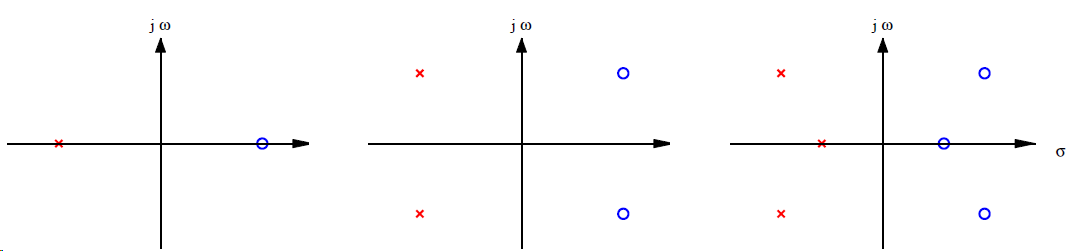
\includegraphics[width=0.8\columnwidth]{Images/allpass}
\end{center}

\noindent Als Merkmal besitzen \textbf{Minimalphasennetzwerke} keine Nullstellen in der RHE.\script{221}\\

\noindent \textbf{Allpol, Allpolfilter} oder auch \textbf{Allpolnetzwerke} haben keine endlichen Nullstellen.
\subsection{Bode-Diagramm}
\subsubsection{Approximation von Bode-Diagramm}
Siehe Kapitel \ref{approx_bode}

\subsubsection{Stabilität}
Wenn ein offener Regelkreis $H(s)$ Pole in der linken s-Halbebene hat (und höchstens zwei Pole im Ursprung bei $s=0$), so ist der geschlossene Regelkreis genau dann asymptotisch stabil, wenn $H(j\omega)$ für die Durchgangsfrequenz $\omega_D$ bei der die Amplitude $20\log_{10}(\left|j\omega_D\right|) = 0dB$ und eine Phase $> -\pi$ hat \script{248}. Siehe auch \script{248} für Phasen- und Amplitudenrand.

\subsubsection{PN-Diagramm to Bode}
Um ein Pol/Nullstellendiagramm zu einem Bode-Diagramm zu transformieren, nach folgenden Punkten vorgehen:
\begin{enumerate}[nosep]
	\item Schlusssteigung = (Anzahl Nullstellen - Anzahl Polstellen) $\cdot 20\frac{dB}{Dek}$
	\item \begin{itemize}[nosep]
		\item Pro Nullstelle im Ursprung steigt die Amplitude bei tiefen Frequenzen um $20\dfrac{dB}{Dek}$
		\item Pro Polstelle im Ursprung fällt die Amplitude bei tiefen Frequenzen um  $20\dfrac{dB}{Dek}$
		\item Sind keine Pol/Nullstellen im Ursprung, hat es bei tiefen Frequenzen keine Steigung
	\end{itemize}
	\item Sobald im Amplitudengang überschwinger drin sind, müssen im Pol-Nullstellendiagramm konjugiert-komplexe Pol-Nullstellen vorkommen.
\end{enumerate}

Für \textbf{Betrag} $|H(j\omega_0)|$ und \textbf{Phase} $\theta$ ergibt dies \script{216}:
\[
	|H(j\omega_0)| = K \cdot \frac{\prod\limits_{i=1}^{m}\overbrace{(j\omega_0 - z_i)}^{A_{z_i}}}{\prod\limits_{j=1}^{n}\underbrace{(j\omega_0 - p_j)}_{A_{p_j}}} \qquad
	\theta(\omega_0) = K + \sum_{i=1}^{m}\theta_{z_i}+ \sum_{j=1}^{m}\theta_{p_j}
\]
\begin{center}
	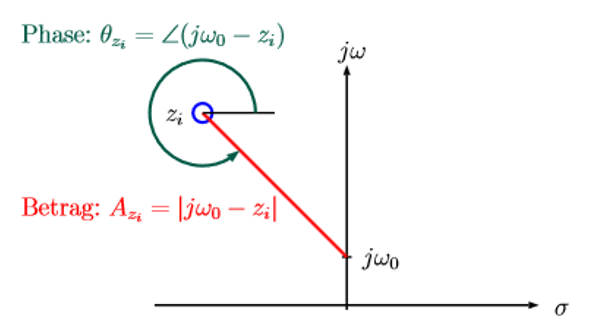
\includegraphics[width=0.5\columnwidth]{Images/pn-to-bode}
\end{center}


\subsection{Nyquist-Diagramm (Orskurve)}
Im Gegensatz zum Bode-Diagramm wird beim Nyquist-Diagramm Betrag und Phase in einem Diagramm gezeichnet. Dazu wird Real- und Imaginärteil in der komplexen Zahlenebene gezeichnet wird.

\subsubsection{Stabilität}
System ist Stabil, solange die Kurve den Punkt $(-1, 0)$ links liegen lässt.
